\documentclass{article} % For LaTeX2e
\usepackage{iclr2022_conference,times}
% Optional math commands from https://github.com/goodfeli/dlbook_notation.
%%%%% NEW MATH DEFINITIONS %%%%%

\usepackage{amsmath,amsfonts,bm}

% Mark sections of captions for referring to divisions of figures
\newcommand{\figleft}{{\em (Left)}}
\newcommand{\figcenter}{{\em (Center)}}
\newcommand{\figright}{{\em (Right)}}
\newcommand{\figtop}{{\em (Top)}}
\newcommand{\figbottom}{{\em (Bottom)}}
\newcommand{\captiona}{{\em (a)}}
\newcommand{\captionb}{{\em (b)}}
\newcommand{\captionc}{{\em (c)}}
\newcommand{\captiond}{{\em (d)}}

% Highlight a newly defined term
\newcommand{\newterm}[1]{{\bf #1}}


% Figure reference, lower-case.
\def\figref#1{figure~\ref{#1}}
% Figure reference, capital. For start of sentence
\def\Figref#1{Figure~\ref{#1}}
\def\twofigref#1#2{figures \ref{#1} and \ref{#2}}
\def\quadfigref#1#2#3#4{figures \ref{#1}, \ref{#2}, \ref{#3} and \ref{#4}}
% Section reference, lower-case.
\def\secref#1{section~\ref{#1}}
% Section reference, capital.
\def\Secref#1{Section~\ref{#1}}
% Reference to two sections.
\def\twosecrefs#1#2{sections \ref{#1} and \ref{#2}}
% Reference to three sections.
\def\secrefs#1#2#3{sections \ref{#1}, \ref{#2} and \ref{#3}}
% Reference to an equation, lower-case.
\def\eqref#1{equation~\ref{#1}}
% Reference to an equation, upper case
\def\Eqref#1{Equation~\ref{#1}}
% A raw reference to an equation---avoid using if possible
\def\plaineqref#1{\ref{#1}}
% Reference to a chapter, lower-case.
\def\chapref#1{chapter~\ref{#1}}
% Reference to an equation, upper case.
\def\Chapref#1{Chapter~\ref{#1}}
% Reference to a range of chapters
\def\rangechapref#1#2{chapters\ref{#1}--\ref{#2}}
% Reference to an algorithm, lower-case.
\def\algref#1{algorithm~\ref{#1}}
% Reference to an algorithm, upper case.
\def\Algref#1{Algorithm~\ref{#1}}
\def\twoalgref#1#2{algorithms \ref{#1} and \ref{#2}}
\def\Twoalgref#1#2{Algorithms \ref{#1} and \ref{#2}}
% Reference to a part, lower case
\def\partref#1{part~\ref{#1}}
% Reference to a part, upper case
\def\Partref#1{Part~\ref{#1}}
\def\twopartref#1#2{parts \ref{#1} and \ref{#2}}

\def\ceil#1{\lceil #1 \rceil}
\def\floor#1{\lfloor #1 \rfloor}
\def\1{\bm{1}}
\newcommand{\train}{\mathcal{D}}
\newcommand{\valid}{\mathcal{D_{\mathrm{valid}}}}
\newcommand{\test}{\mathcal{D_{\mathrm{test}}}}

\def\eps{{\epsilon}}


% Random variables
\def\reta{{\textnormal{$\eta$}}}
\def\ra{{\textnormal{a}}}
\def\rb{{\textnormal{b}}}
\def\rc{{\textnormal{c}}}
\def\rd{{\textnormal{d}}}
\def\re{{\textnormal{e}}}
\def\rf{{\textnormal{f}}}
\def\rg{{\textnormal{g}}}
\def\rh{{\textnormal{h}}}
\def\ri{{\textnormal{i}}}
\def\rj{{\textnormal{j}}}
\def\rk{{\textnormal{k}}}
\def\rl{{\textnormal{l}}}
% rm is already a command, just don't name any random variables m
\def\rn{{\textnormal{n}}}
\def\ro{{\textnormal{o}}}
\def\rp{{\textnormal{p}}}
\def\rq{{\textnormal{q}}}
\def\rr{{\textnormal{r}}}
\def\rs{{\textnormal{s}}}
\def\rt{{\textnormal{t}}}
\def\ru{{\textnormal{u}}}
\def\rv{{\textnormal{v}}}
\def\rw{{\textnormal{w}}}
\def\rx{{\textnormal{x}}}
\def\ry{{\textnormal{y}}}
\def\rz{{\textnormal{z}}}

% Random vectors
\def\rvepsilon{{\mathbf{\epsilon}}}
\def\rvtheta{{\mathbf{\theta}}}
\def\rva{{\mathbf{a}}}
\def\rvb{{\mathbf{b}}}
\def\rvc{{\mathbf{c}}}
\def\rvd{{\mathbf{d}}}
\def\rve{{\mathbf{e}}}
\def\rvf{{\mathbf{f}}}
\def\rvg{{\mathbf{g}}}
\def\rvh{{\mathbf{h}}}
\def\rvu{{\mathbf{i}}}
\def\rvj{{\mathbf{j}}}
\def\rvk{{\mathbf{k}}}
\def\rvl{{\mathbf{l}}}
\def\rvm{{\mathbf{m}}}
\def\rvn{{\mathbf{n}}}
\def\rvo{{\mathbf{o}}}
\def\rvp{{\mathbf{p}}}
\def\rvq{{\mathbf{q}}}
\def\rvr{{\mathbf{r}}}
\def\rvs{{\mathbf{s}}}
\def\rvt{{\mathbf{t}}}
\def\rvu{{\mathbf{u}}}
\def\rvv{{\mathbf{v}}}
\def\rvw{{\mathbf{w}}}
\def\rvx{{\mathbf{x}}}
\def\rvy{{\mathbf{y}}}
\def\rvz{{\mathbf{z}}}

% Elements of random vectors
\def\erva{{\textnormal{a}}}
\def\ervb{{\textnormal{b}}}
\def\ervc{{\textnormal{c}}}
\def\ervd{{\textnormal{d}}}
\def\erve{{\textnormal{e}}}
\def\ervf{{\textnormal{f}}}
\def\ervg{{\textnormal{g}}}
\def\ervh{{\textnormal{h}}}
\def\ervi{{\textnormal{i}}}
\def\ervj{{\textnormal{j}}}
\def\ervk{{\textnormal{k}}}
\def\ervl{{\textnormal{l}}}
\def\ervm{{\textnormal{m}}}
\def\ervn{{\textnormal{n}}}
\def\ervo{{\textnormal{o}}}
\def\ervp{{\textnormal{p}}}
\def\ervq{{\textnormal{q}}}
\def\ervr{{\textnormal{r}}}
\def\ervs{{\textnormal{s}}}
\def\ervt{{\textnormal{t}}}
\def\ervu{{\textnormal{u}}}
\def\ervv{{\textnormal{v}}}
\def\ervw{{\textnormal{w}}}
\def\ervx{{\textnormal{x}}}
\def\ervy{{\textnormal{y}}}
\def\ervz{{\textnormal{z}}}

% Random matrices
\def\rmA{{\mathbf{A}}}
\def\rmB{{\mathbf{B}}}
\def\rmC{{\mathbf{C}}}
\def\rmD{{\mathbf{D}}}
\def\rmE{{\mathbf{E}}}
\def\rmF{{\mathbf{F}}}
\def\rmG{{\mathbf{G}}}
\def\rmH{{\mathbf{H}}}
\def\rmI{{\mathbf{I}}}
\def\rmJ{{\mathbf{J}}}
\def\rmK{{\mathbf{K}}}
\def\rmL{{\mathbf{L}}}
\def\rmM{{\mathbf{M}}}
\def\rmN{{\mathbf{N}}}
\def\rmO{{\mathbf{O}}}
\def\rmP{{\mathbf{P}}}
\def\rmQ{{\mathbf{Q}}}
\def\rmR{{\mathbf{R}}}
\def\rmS{{\mathbf{S}}}
\def\rmT{{\mathbf{T}}}
\def\rmU{{\mathbf{U}}}
\def\rmV{{\mathbf{V}}}
\def\rmW{{\mathbf{W}}}
\def\rmX{{\mathbf{X}}}
\def\rmY{{\mathbf{Y}}}
\def\rmZ{{\mathbf{Z}}}

% Elements of random matrices
\def\ermA{{\textnormal{A}}}
\def\ermB{{\textnormal{B}}}
\def\ermC{{\textnormal{C}}}
\def\ermD{{\textnormal{D}}}
\def\ermE{{\textnormal{E}}}
\def\ermF{{\textnormal{F}}}
\def\ermG{{\textnormal{G}}}
\def\ermH{{\textnormal{H}}}
\def\ermI{{\textnormal{I}}}
\def\ermJ{{\textnormal{J}}}
\def\ermK{{\textnormal{K}}}
\def\ermL{{\textnormal{L}}}
\def\ermM{{\textnormal{M}}}
\def\ermN{{\textnormal{N}}}
\def\ermO{{\textnormal{O}}}
\def\ermP{{\textnormal{P}}}
\def\ermQ{{\textnormal{Q}}}
\def\ermR{{\textnormal{R}}}
\def\ermS{{\textnormal{S}}}
\def\ermT{{\textnormal{T}}}
\def\ermU{{\textnormal{U}}}
\def\ermV{{\textnormal{V}}}
\def\ermW{{\textnormal{W}}}
\def\ermX{{\textnormal{X}}}
\def\ermY{{\textnormal{Y}}}
\def\ermZ{{\textnormal{Z}}}

% Vectors
\def\vzero{{\bm{0}}}
\def\vone{{\bm{1}}}
\def\vmu{{\bm{\mu}}}
\def\vtheta{{\bm{\theta}}}
\def\va{{\bm{a}}}
\def\vb{{\bm{b}}}
\def\vc{{\bm{c}}}
\def\vd{{\bm{d}}}
\def\ve{{\bm{e}}}
\def\vf{{\bm{f}}}
\def\vg{{\bm{g}}}
\def\vh{{\bm{h}}}
\def\vi{{\bm{i}}}
\def\vj{{\bm{j}}}
\def\vk{{\bm{k}}}
\def\vl{{\bm{l}}}
\def\vm{{\bm{m}}}
\def\vn{{\bm{n}}}
\def\vo{{\bm{o}}}
\def\vp{{\bm{p}}}
\def\vq{{\bm{q}}}
\def\vr{{\bm{r}}}
\def\vs{{\bm{s}}}
\def\vt{{\bm{t}}}
\def\vu{{\bm{u}}}
\def\vv{{\bm{v}}}
\def\vw{{\bm{w}}}
\def\vx{{\bm{x}}}
\def\vy{{\bm{y}}}
\def\vz{{\bm{z}}}

% Elements of vectors
\def\evalpha{{\alpha}}
\def\evbeta{{\beta}}
\def\evepsilon{{\epsilon}}
\def\evlambda{{\lambda}}
\def\evomega{{\omega}}
\def\evmu{{\mu}}
\def\evpsi{{\psi}}
\def\evsigma{{\sigma}}
\def\evtheta{{\theta}}
\def\eva{{a}}
\def\evb{{b}}
\def\evc{{c}}
\def\evd{{d}}
\def\eve{{e}}
\def\evf{{f}}
\def\evg{{g}}
\def\evh{{h}}
\def\evi{{i}}
\def\evj{{j}}
\def\evk{{k}}
\def\evl{{l}}
\def\evm{{m}}
\def\evn{{n}}
\def\evo{{o}}
\def\evp{{p}}
\def\evq{{q}}
\def\evr{{r}}
\def\evs{{s}}
\def\evt{{t}}
\def\evu{{u}}
\def\evv{{v}}
\def\evw{{w}}
\def\evx{{x}}
\def\evy{{y}}
\def\evz{{z}}

% Matrix
\def\mA{{\bm{A}}}
\def\mB{{\bm{B}}}
\def\mC{{\bm{C}}}
\def\mD{{\bm{D}}}
\def\mE{{\bm{E}}}
\def\mF{{\bm{F}}}
\def\mG{{\bm{G}}}
\def\mH{{\bm{H}}}
\def\mI{{\bm{I}}}
\def\mJ{{\bm{J}}}
\def\mK{{\bm{K}}}
\def\mL{{\bm{L}}}
\def\mM{{\bm{M}}}
\def\mN{{\bm{N}}}
\def\mO{{\bm{O}}}
\def\mP{{\bm{P}}}
\def\mQ{{\bm{Q}}}
\def\mR{{\bm{R}}}
\def\mS{{\bm{S}}}
\def\mT{{\bm{T}}}
\def\mU{{\bm{U}}}
\def\mV{{\bm{V}}}
\def\mW{{\bm{W}}}
\def\mX{{\bm{X}}}
\def\mY{{\bm{Y}}}
\def\mZ{{\bm{Z}}}
\def\mBeta{{\bm{\beta}}}
\def\mPhi{{\bm{\Phi}}}
\def\mLambda{{\bm{\Lambda}}}
\def\mSigma{{\bm{\Sigma}}}

% Tensor
\DeclareMathAlphabet{\mathsfit}{\encodingdefault}{\sfdefault}{m}{sl}
\SetMathAlphabet{\mathsfit}{bold}{\encodingdefault}{\sfdefault}{bx}{n}
\newcommand{\tens}[1]{\bm{\mathsfit{#1}}}
\def\tA{{\tens{A}}}
\def\tB{{\tens{B}}}
\def\tC{{\tens{C}}}
\def\tD{{\tens{D}}}
\def\tE{{\tens{E}}}
\def\tF{{\tens{F}}}
\def\tG{{\tens{G}}}
\def\tH{{\tens{H}}}
\def\tI{{\tens{I}}}
\def\tJ{{\tens{J}}}
\def\tK{{\tens{K}}}
\def\tL{{\tens{L}}}
\def\tM{{\tens{M}}}
\def\tN{{\tens{N}}}
\def\tO{{\tens{O}}}
\def\tP{{\tens{P}}}
\def\tQ{{\tens{Q}}}
\def\tR{{\tens{R}}}
\def\tS{{\tens{S}}}
\def\tT{{\tens{T}}}
\def\tU{{\tens{U}}}
\def\tV{{\tens{V}}}
\def\tW{{\tens{W}}}
\def\tX{{\tens{X}}}
\def\tY{{\tens{Y}}}
\def\tZ{{\tens{Z}}}


% Graph
\def\gA{{\mathcal{A}}}
\def\gB{{\mathcal{B}}}
\def\gC{{\mathcal{C}}}
\def\gD{{\mathcal{D}}}
\def\gE{{\mathcal{E}}}
\def\gF{{\mathcal{F}}}
\def\gG{{\mathcal{G}}}
\def\gH{{\mathcal{H}}}
\def\gI{{\mathcal{I}}}
\def\gJ{{\mathcal{J}}}
\def\gK{{\mathcal{K}}}
\def\gL{{\mathcal{L}}}
\def\gM{{\mathcal{M}}}
\def\gN{{\mathcal{N}}}
\def\gO{{\mathcal{O}}}
\def\gP{{\mathcal{P}}}
\def\gQ{{\mathcal{Q}}}
\def\gR{{\mathcal{R}}}
\def\gS{{\mathcal{S}}}
\def\gT{{\mathcal{T}}}
\def\gU{{\mathcal{U}}}
\def\gV{{\mathcal{V}}}
\def\gW{{\mathcal{W}}}
\def\gX{{\mathcal{X}}}
\def\gY{{\mathcal{Y}}}
\def\gZ{{\mathcal{Z}}}

% Sets
\def\sA{{\mathbb{A}}}
\def\sB{{\mathbb{B}}}
\def\sC{{\mathbb{C}}}
\def\sD{{\mathbb{D}}}
% Don't use a set called E, because this would be the same as our symbol
% for expectation.
\def\sF{{\mathbb{F}}}
\def\sG{{\mathbb{G}}}
\def\sH{{\mathbb{H}}}
\def\sI{{\mathbb{I}}}
\def\sJ{{\mathbb{J}}}
\def\sK{{\mathbb{K}}}
\def\sL{{\mathbb{L}}}
\def\sM{{\mathbb{M}}}
\def\sN{{\mathbb{N}}}
\def\sO{{\mathbb{O}}}
\def\sP{{\mathbb{P}}}
\def\sQ{{\mathbb{Q}}}
\def\sR{{\mathbb{R}}}
\def\sS{{\mathbb{S}}}
\def\sT{{\mathbb{T}}}
\def\sU{{\mathbb{U}}}
\def\sV{{\mathbb{V}}}
\def\sW{{\mathbb{W}}}
\def\sX{{\mathbb{X}}}
\def\sY{{\mathbb{Y}}}
\def\sZ{{\mathbb{Z}}}

% Entries of a matrix
\def\emLambda{{\Lambda}}
\def\emA{{A}}
\def\emB{{B}}
\def\emC{{C}}
\def\emD{{D}}
\def\emE{{E}}
\def\emF{{F}}
\def\emG{{G}}
\def\emH{{H}}
\def\emI{{I}}
\def\emJ{{J}}
\def\emK{{K}}
\def\emL{{L}}
\def\emM{{M}}
\def\emN{{N}}
\def\emO{{O}}
\def\emP{{P}}
\def\emQ{{Q}}
\def\emR{{R}}
\def\emS{{S}}
\def\emT{{T}}
\def\emU{{U}}
\def\emV{{V}}
\def\emW{{W}}
\def\emX{{X}}
\def\emY{{Y}}
\def\emZ{{Z}}
\def\emSigma{{\Sigma}}

% entries of a tensor
% Same font as tensor, without \bm wrapper
\newcommand{\etens}[1]{\mathsfit{#1}}
\def\etLambda{{\etens{\Lambda}}}
\def\etA{{\etens{A}}}
\def\etB{{\etens{B}}}
\def\etC{{\etens{C}}}
\def\etD{{\etens{D}}}
\def\etE{{\etens{E}}}
\def\etF{{\etens{F}}}
\def\etG{{\etens{G}}}
\def\etH{{\etens{H}}}
\def\etI{{\etens{I}}}
\def\etJ{{\etens{J}}}
\def\etK{{\etens{K}}}
\def\etL{{\etens{L}}}
\def\etM{{\etens{M}}}
\def\etN{{\etens{N}}}
\def\etO{{\etens{O}}}
\def\etP{{\etens{P}}}
\def\etQ{{\etens{Q}}}
\def\etR{{\etens{R}}}
\def\etS{{\etens{S}}}
\def\etT{{\etens{T}}}
\def\etU{{\etens{U}}}
\def\etV{{\etens{V}}}
\def\etW{{\etens{W}}}
\def\etX{{\etens{X}}}
\def\etY{{\etens{Y}}}
\def\etZ{{\etens{Z}}}

% The true underlying data generating distribution
\newcommand{\pdata}{p_{\rm{data}}}
% The empirical distribution defined by the training set
\newcommand{\ptrain}{\hat{p}_{\rm{data}}}
\newcommand{\Ptrain}{\hat{P}_{\rm{data}}}
% The model distribution
\newcommand{\pmodel}{p_{\rm{model}}}
\newcommand{\Pmodel}{P_{\rm{model}}}
\newcommand{\ptildemodel}{\tilde{p}_{\rm{model}}}
% Stochastic autoencoder distributions
\newcommand{\pencode}{p_{\rm{encoder}}}
\newcommand{\pdecode}{p_{\rm{decoder}}}
\newcommand{\precons}{p_{\rm{reconstruct}}}

\newcommand{\laplace}{\mathrm{Laplace}} % Laplace distribution

\newcommand{\E}{\mathbb{E}}
\newcommand{\Ls}{\mathcal{L}}
\newcommand{\R}{\mathbb{R}}
\newcommand{\emp}{\tilde{p}}
\newcommand{\lr}{\alpha}
\newcommand{\reg}{\lambda}
\newcommand{\rect}{\mathrm{rectifier}}
\newcommand{\softmax}{\mathrm{softmax}}
\newcommand{\sigmoid}{\sigma}
\newcommand{\softplus}{\zeta}
\newcommand{\KL}{D_{\mathrm{KL}}}
\newcommand{\Var}{\mathrm{Var}}
\newcommand{\standarderror}{\mathrm{SE}}
\newcommand{\Cov}{\mathrm{Cov}}
% Wolfram Mathworld says $L^2$ is for function spaces and $\ell^2$ is for vectors
% But then they seem to use $L^2$ for vectors throughout the site, and so does
% wikipedia.
\newcommand{\normlzero}{L^0}
\newcommand{\normlone}{L^1}
\newcommand{\normltwo}{L^2}
\newcommand{\normlp}{L^p}
\newcommand{\normmax}{L^\infty}

\newcommand{\parents}{Pa} % See usage in notation.tex. Chosen to match Daphne's book.

\DeclareMathOperator*{\argmax}{arg\,max}
\DeclareMathOperator*{\argmin}{arg\,min}

\DeclareMathOperator{\sign}{sign}
\DeclareMathOperator{\Tr}{Tr}
\let\ab\allowbreak


%######## APS360: Uncomment your submission name
\newcommand{\apsname}{Project Proposal}
%\newcommand{\apsname}{Progress Report}
%\newcommand{\apsname}{Final Report}

%######## APS360: Put your Group Number here
\newcommand{\gpnumber}{28}

\usepackage{hyperref}
\usepackage{url}
\usepackage{graphicx}


%######## APS360: Put your project Title here
\title{Project Progress Report: Traffic Sign Recognition Through Deep Learning}


%######## APS360: Put your names, student IDs and Emails here
\author{Salwa Waseem  \\
Student\# 10090214161\\
\texttt{salwa.waseem@mail.utoronto.ca} \\
\And
Maya Ramaneetharan Ramanathan  \\
Student\# 1008717596 \\
\texttt{maya.ramanathan@mail.utoronto.ca} \\
\AND
Maryah Noorani  \\
Student\# 1008343188 \\
\texttt{maryah.noorani@mail.utoronto.ca} \\
\And
Seoyeon (Sally) Kim \\
Student\# 1007713949 \\
\texttt{sysally.kim@mail.utoronto.ca} \\
\AND
}

% The \author macro works with any number of authors. There are two commands
% used to separate the names and addresses of multiple authors: \And and \AND.
%
% Using \And between authors leaves it to \LaTeX{} to determine where to break
% the lines. Using \AND forces a linebreak at that point. So, if \LaTeX{}
% puts 3 of 4 authors names on the first line, and the last on the second
% line, try using \AND instead of \And before the third author name.

\newcommand{\fix}{\marginpar{FIX}}
\newcommand{\new}{\marginpar{NEW}}

\iclrfinalcopy 
%######## APS360: Document starts here
\begin{document}


\maketitle

\begin{abstract}
%This template should be used for all your project related reports in APS360 course. -- Write an abstract for your project here. Please review the \textbf{ First Course Tutorial} for a quick start

The following document is a progress report outlining the developments made in the Traffic Sign Recognition (TSR) Project. A Convolutional Neural Network (CNN) has been employed along with a Support Vector Machines (SVM) to classify various traffic signs drivers may encounter on the road. Traffic Signs utilized to train the model are found in the German Traffic Sign Recognition Benchmark (GTSRD) and have been supplemented by various traffic signs found specifically in Toronto by the team. These photos have been passed into the baseline and primary model and received a high accuracy with the allocated training set. This document also outlines the contributions made by each member to the overall creation and testing of the model. 


%######## APS360: Do not change the next line. This shows your Main body page count.
----Total Pages: \pageref{last_page}
\end{abstract}

\section{Brief Project Description}
Traffic Sign Recognition (TSR) is a crucial asset in driver-assistance systems. They are utilised to improve road safety by automating detection of traffic signs. This is essential to ensure vehicles are responsive to speed warnings, road conditions and are ultimately adaptable to dynamic driving environments. This technology aims to improve safety in vehicles to reduce human error and eventually mitigate road accidents. However, there are several challenges due to assorted lighting conditions, weather, and overall accuracy of interpretation. 

This project intends to generalize TSR across complex driving conditions while retaining recognition accuracy and computational efficiency. To achieve this, TSR models utilize deep learning models and algorithms to enhance classification performance. Deep learning is leveraged in this study as it is highly adaptable feature learning and is incredibly adept at scaling to large datasets. Ultimately, this deep learning model can be trained to effectively and accurately identify traffic signs, thus creating a safer driving environment. 

\newpage

\begin{figure}[h]
\begin{center}
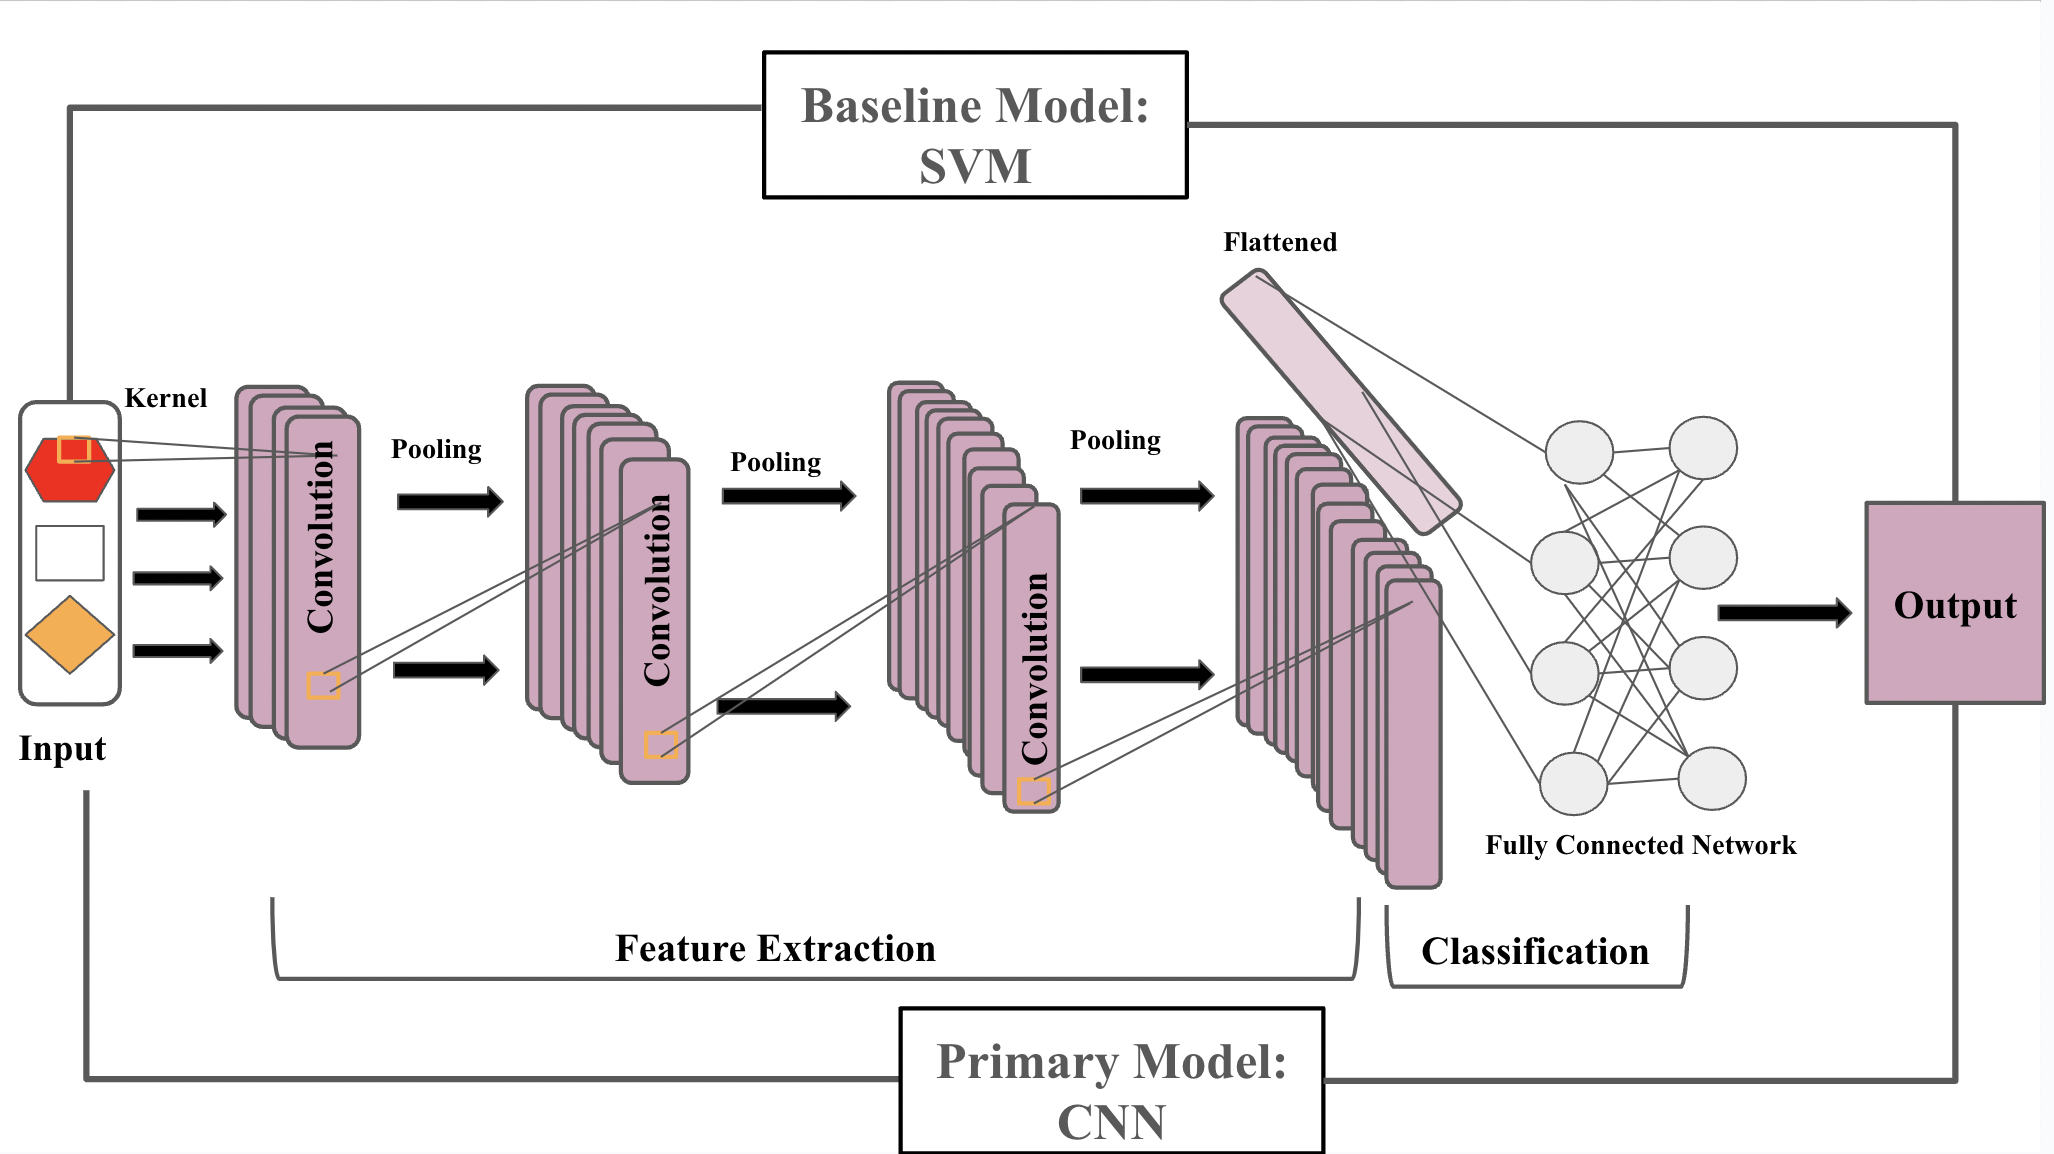
\includegraphics[width=\textwidth]{Figs/project_desc.png}
\end{center}
\caption{Schematic of Deep Learning Model }
\end{figure} 


\section{Individual Contributions and Responsibilities}
Through our weekly meetings, held weekly on Thursdays at 2pm, there has been effective collaboration amongst the team to create models and test the model through training sets. Each member is expected to contribute to brainstorming sessions, code development and most importantly, update with any completed tasks or reporting any uncertainties that may have hindered completion of a task or absence to a meeting. Meetings have been held in person to mitigate code overwriting. 

The team also has a group chat via Instagram DMs to communicate any update or issues. Links to meetings, references and any other resources to supplement the project are also shared in this group chat. The baseline model and primary model have been developed on Google Colab, where each team member has access to it and stored among a shared Google Drive. Github has also been employed to store notebooks and any vital documents for reference. 
There is an emphasis on equality of work distribution in this team. While all tasks have been fleshed out in Table 1, emergencies can occur and therefore contingencies have been put into place to ensure tasks get completed. For example, if any task is incomplete, a meeting will be held to discuss the situation and work will be reallocated accordingly. 

\begin{table}[h]
    \centering
    \begin{tabular}{cccc}
         Assignment &  Task &  Assigned To & Deadline \\
         Progress Report&&&\\
         Written Document &  Project Description&  Salwa & 03/11/2024\\
         &  Individual Contributions &  Salwa & 03/11/2024\\
         &  Data Processing &  Maya & 03/11/2024\\
         &  Baseline Model &  Sally & 03/11/2024\\
         &  Primary Model &  Maryah & 03/11/2024\\
         Data Processing &  Data Search &  Salwa & 03/11/2024\\
 & Data Loading & Sally&03/11/2024\\
         &  Data Cleaning &  Maryah& 03/11/2024\\
         &  Data Mounting &  Maya & 03/11/2024\\
 Baseline Model & Support Vector Machines (SVM) & Sally&03/11/2024\\
 Primary Model & Architecture & Maryah&03/11/2024\\
 & Training & Salwa &03/11/2024\\
 Final Project&&&\\
 Project Final Report & Revising Proposal & All Members &26/11/2024\\
 & Quantitative Results & Maryah &26/11/2024\\
 & Qualitative Results & Sally &26/11/2024\\
 & Validation Set (new data) & Maya &26/11/2024\\
 & Discussion & Salwa&26/11/2024\\
 Project Presentation & Problem and Data & Salwa&28/11/2024\\
 & Data Processing and Model & Maryah&28/11/2024\\
 & Demonstration and Editing & Sally&28/11/2024\\
 & Overall Results and Key Takeaways & Maya &28/11/2024\\
    \end{tabular}
    \caption{Task Breakdown and Timeline}
    \label{tab:my_label}
\end{table}

\section{Notable Contributions}
\subsection{Data Processing}
\subsubsection{Data Collection and Sources:}
The dataset to be used for this model is taken from the German Traffic Sign Recognition Benchmark (GTSRB) which contains pictures captured from the real-world. This diverse dataset includes images of different lighting conditions, angles and backgrounds and each image is labeled according to its corresponding class. This dataset consists of 43 classes and 51,839 images.
\subsubsection{Data Cleaning and Preprocessing:}
A series of preprocessing steps are applied to the dataset to clean and standardize the data going into the model. This includes:
Resizing: All images are resized to 128x128 pixels to standardize the input size across the dataset. 
\begin{itemize}
    \item Normalization: Each image’s pixel value is normalized to fall within the range of [0,1] to ensure the model focuses on all areas of the image equally and to help the model learn properly.
    \item Augmentation: Data augmentation techniques such as rotations, flips, brightness adjustments and zooms have been utilized to increase training data while simultaneously changing the data enough to prevent overfitting. These transformations also simulate the varying conditions of traffic signals in real-world scenarios, better equipping the model for the outside world.
\end{itemize}
\subsubsection{Data Splitting:}
The dataset was split into training, validation, and testing sets with a 70-15-15 split ratio. This means that the 51,839 images were split into 36,287 training images and 2,332 validation images and 2,332 testing images.
\subsubsection{Example Data Samples:}
One example from our cleaned dataset includes the following:
Speed Limit Sign: Here the speed limit sign is in the center of the 128x128 pixel image. There are multiple variations of this same image (data augmentations) to help the model learn without overfitting.


\label{gen_inst}
\begin{figure}[h]
\begin{center}
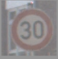
\includegraphics[width=0.15\textwidth]{Figs/Traffic signal (original img).png}
\end{center}
\caption{Original Image size (59x59 pixels)}
\end{figure}

\label{gen_inst}
\begin{figure}[h]
\begin{center}
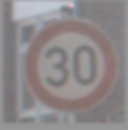
\includegraphics[width=0.25\textwidth]{Figs/Traffic signal (resized img).png}
\end{center}
\caption{Image after resizing (128x128 pixels)}
\end{figure}

\label{gen_inst}
\begin{figure}[h]
\begin{center}
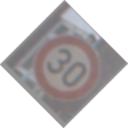
\includegraphics[width=0.35\textwidth]{Figs/rotated 30.png}
\end{center}
\caption{Image after a Data Augmentation (Rotation by 45°)}
\end{figure}



\subsubsection{Plan for New Data Testing:}
To assess the model, we plan to gather new images from an alternate traffic dataset which is not included in our initial training set. This will allow us to evaluate the model’s performance on completely unseen data which will simulate its behavior in the real-world more closely.
\subsubsection{Challenges:}
One challenge faced was the handling of images where the signs were partially covered or inaccessible due to some obstruction. These images required careful cropping and augmentation techniques to successfully detect the label. Additionally, variations in lighting led to inconsistencies in the result. This was handled through normalization and data augmentation. 

\subsection{Baseline Model}
For the baseline model, we implemented a Support Vector Machine (SVM) classifier trained on the processed complete dataset.
An SVM is a supervised machine learning algorithm that classifies data by finding an optimal hyperplane that best separates data points into different classes in a high-dimensional space. For binary classification, this hyperplane is a line that divides data into two groups, maximizing the margin between them. In multiclass classification, an SVM handles multiple classes by creating multiple hyperplanes to separate each class pairwise. Data points closest to the hyperplane, known as support vectors, are particularly important as they define the boundary position and orientation, helping to generalize the model’s predictions\citep{yue2003svm}. Figure 5 models how a SVM would classify the classes.

\newpage
\label{gen_inst}
\begin{figure}[h]
\begin{center}
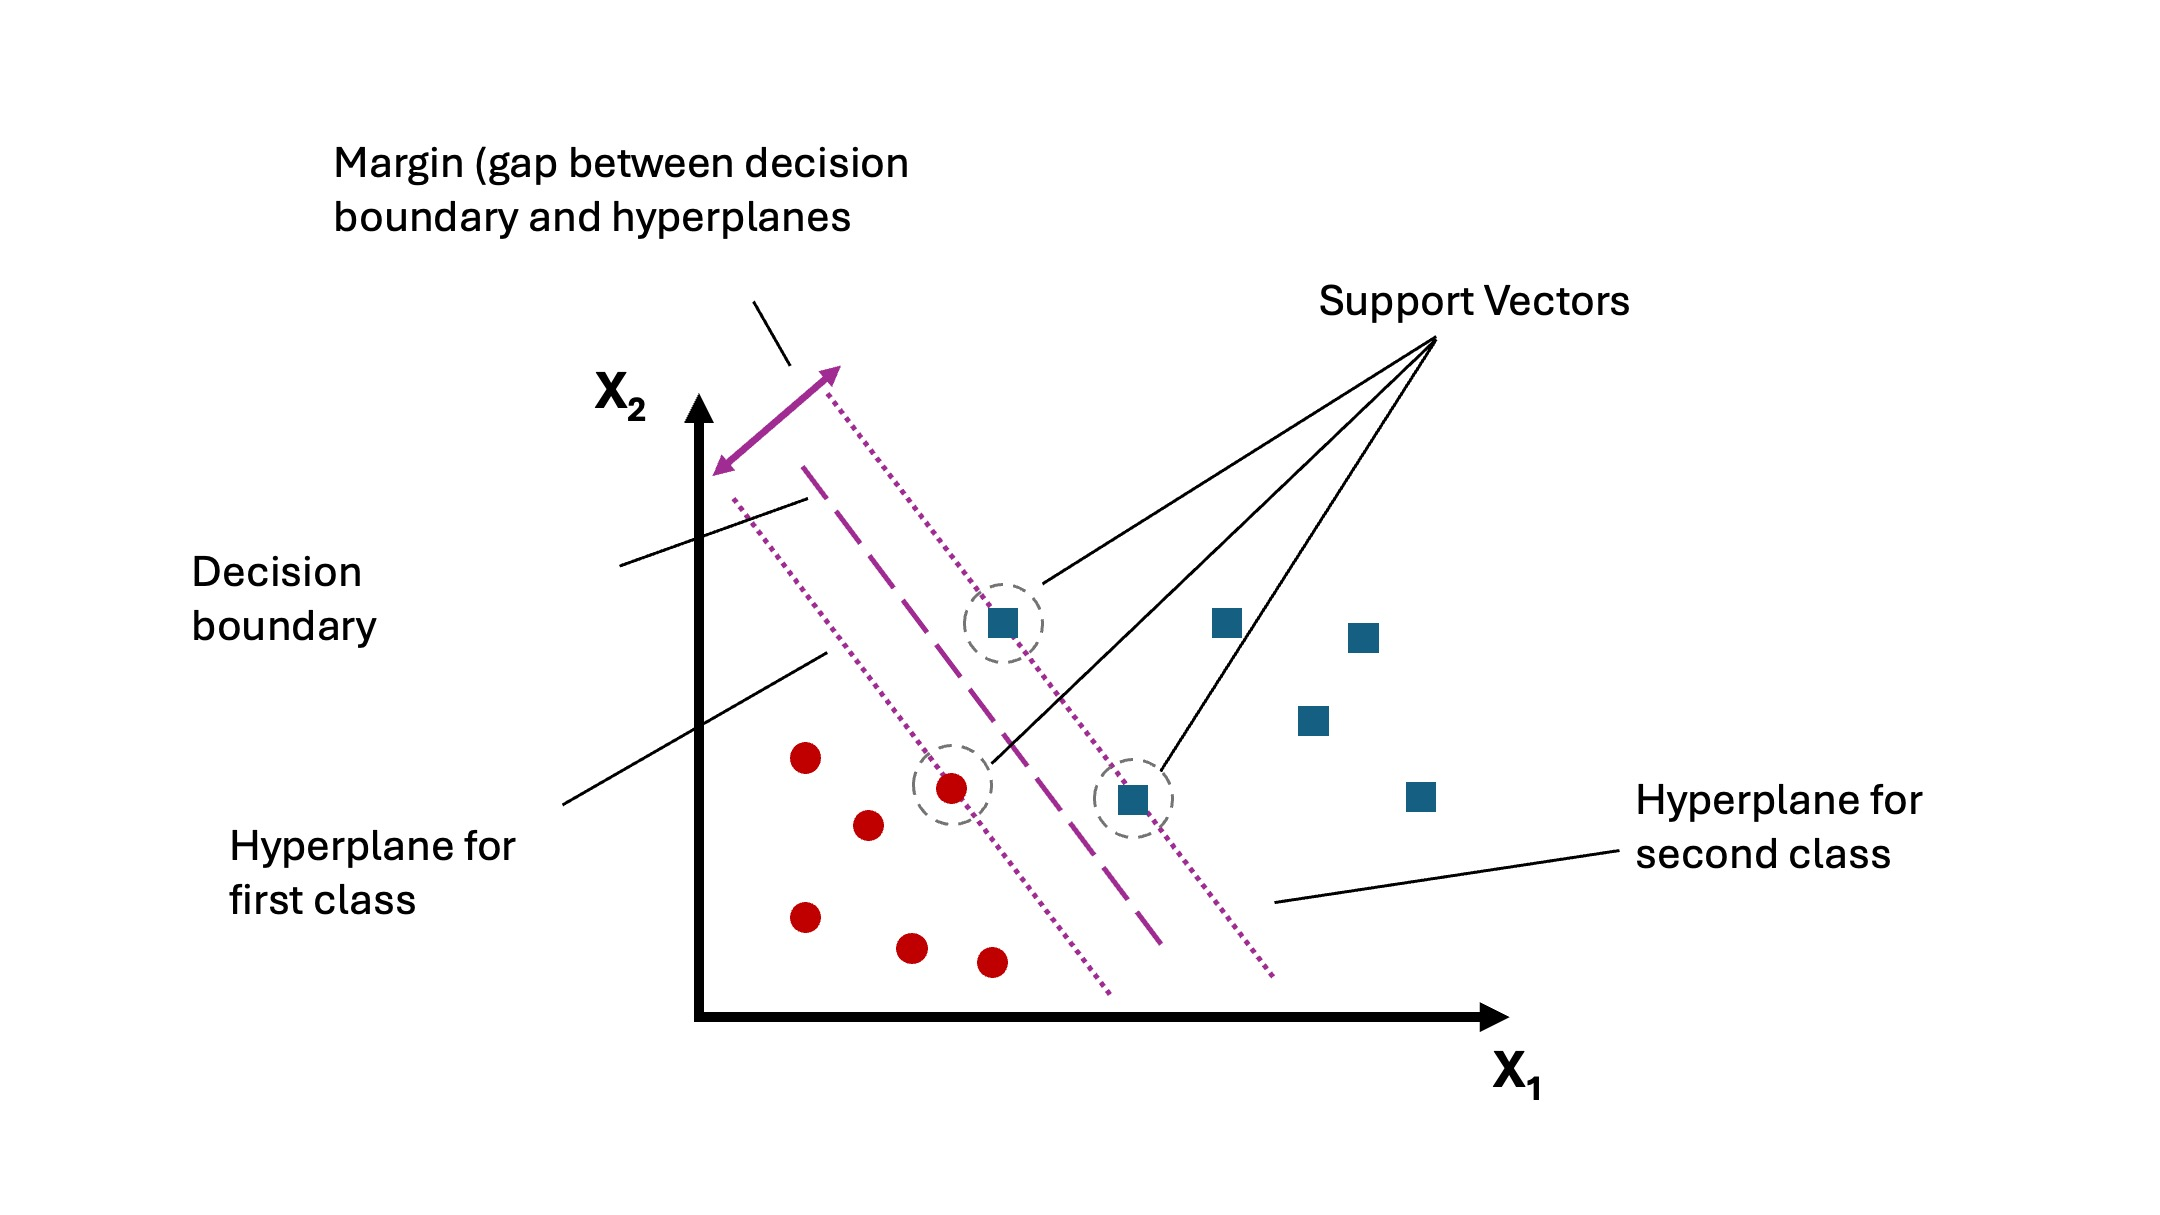
\includegraphics[width=\textwidth]{Figs/Figure_1_for_baseline.jpg}
\end{center}
\caption{How a SVM model separates classes}
\end{figure}

When data isn’t linearly separable, SVM uses a technique called the "kernel trick" to transform the data into a higher-dimensional space, where a linear separation becomes possible. For this baseline model, we used a linear kernel, which balances simplicity with efficiency, and serves as a foundation for understanding initial performance.

The current dataset required some additional preprocessing to make it suitable for the SVM. We resized each image to 32x32 pixels and converted them to grayscale, reducing complexity while preserving the core visual features. The grayscale images were flattened into one-dimensional vectors, allowing the SVM to handle images as structured feature sets. To further optimize model convergence, these vectors were standardized, ensuring uniformity in pixel intensity ranges.

Model evaluation was performed using accuracy, a straightforward metric aligned with the task's objective to classify traffic signs accurately. Our baseline SVM achieved a solid initial accuracy of 84.56\%, showing that even a straightforward linear model can identify important patterns within the traffic sign data. This outcome suggests that SVM provides a reliable baseline, though additional accuracy improvements may be possible by experimenting with non-linear kernels or more complex model structures. A detailed schematic of the SVM model, including the preprocessing steps, classification process, and evaluation metrics, is shown in Figure 6, outlining each stage from data preparation to performance evaluation.

\newpage
\begin{figure}[h]
\begin{center}
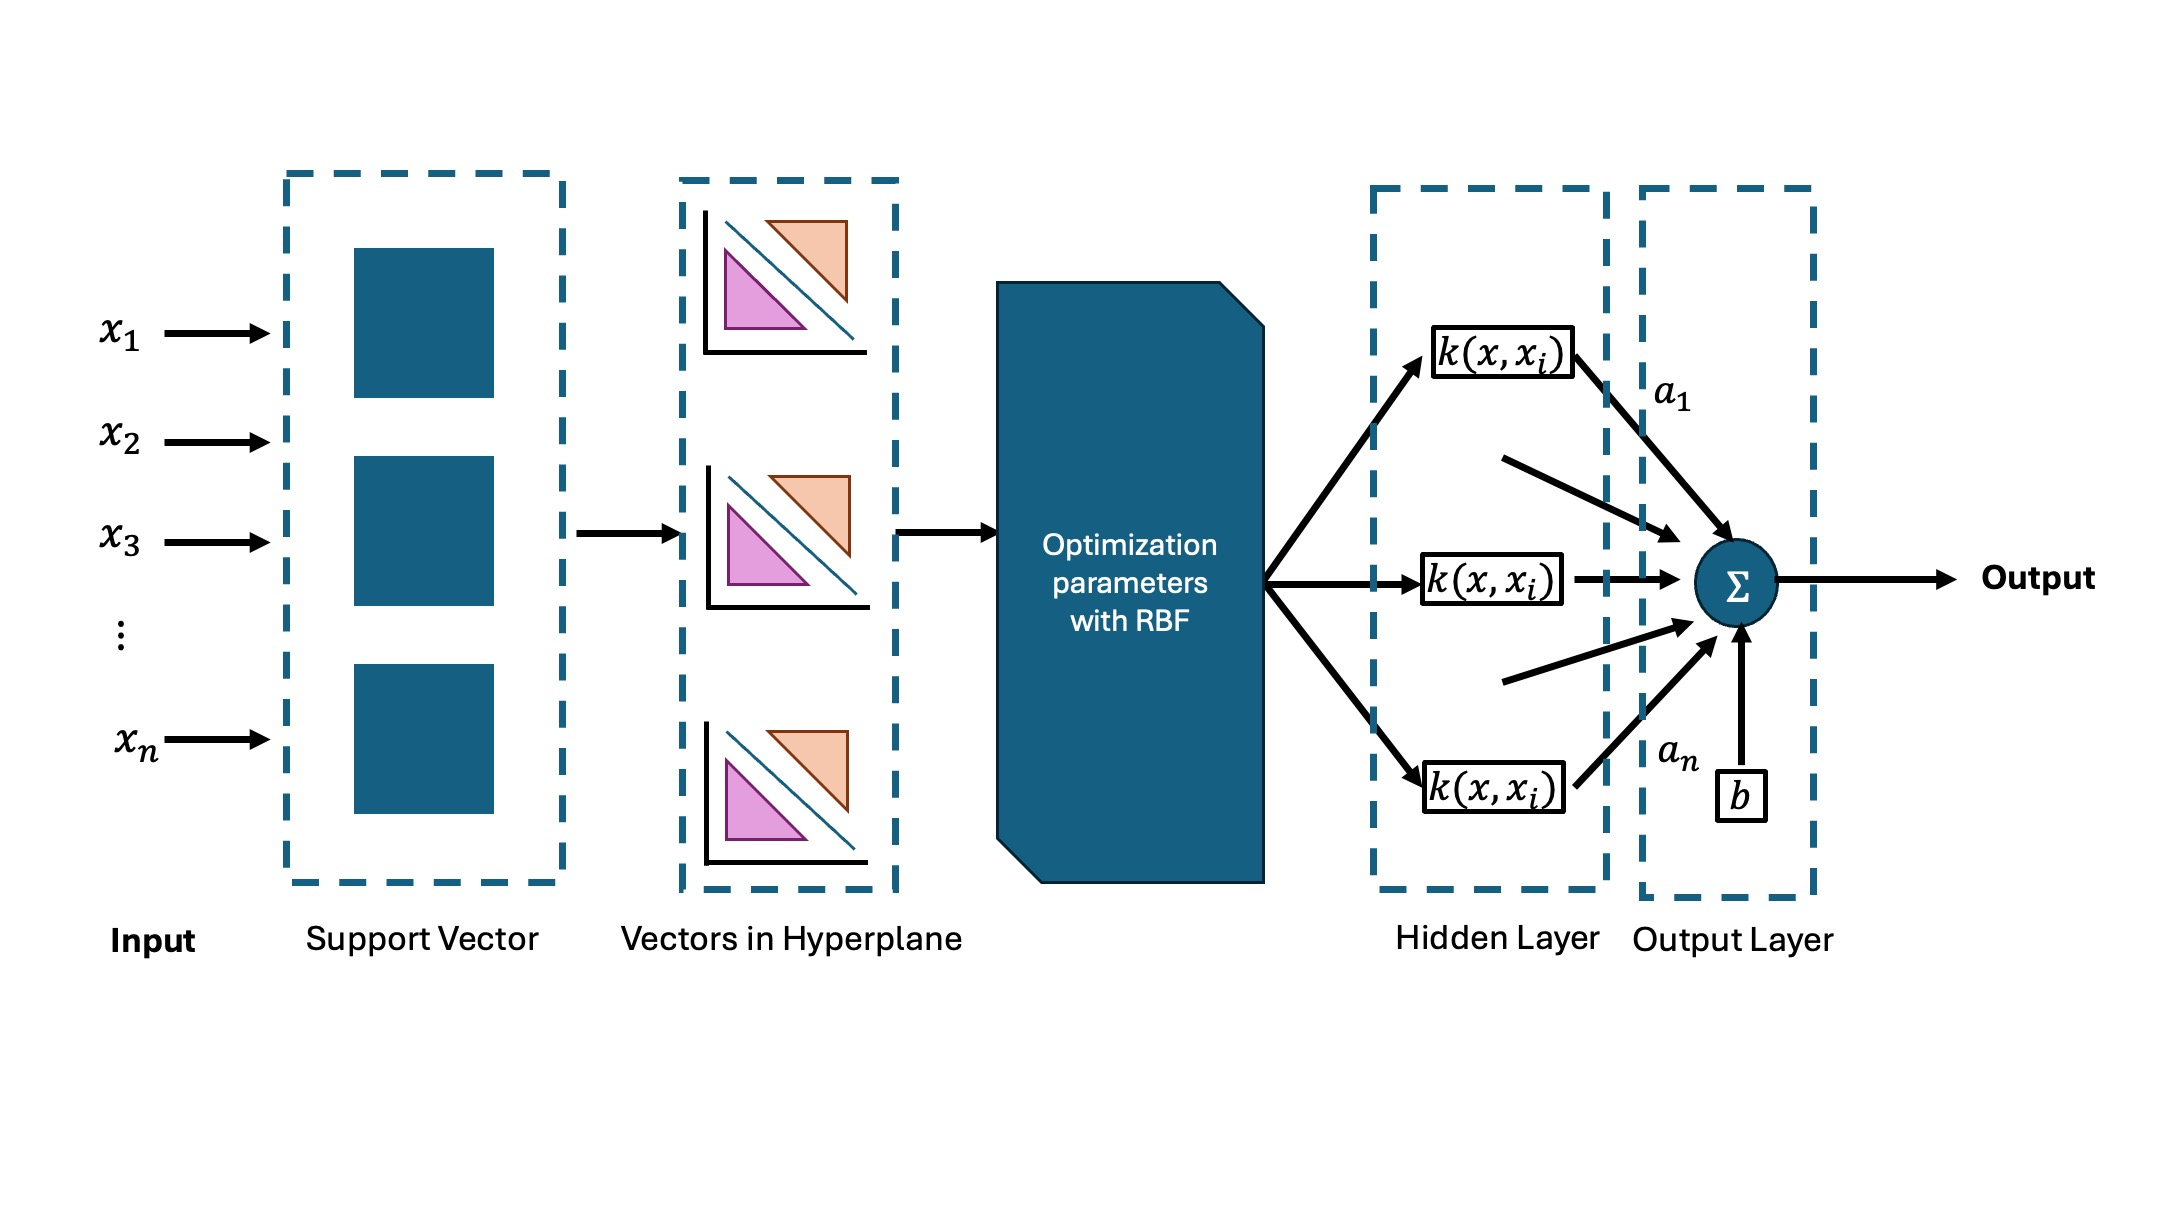
\includegraphics[width=\textwidth]{Figs/Figure_2_for_baseline.jpg}
\end{center}
\caption{Diagram of SVM model}
\end{figure} 


\subsection{Primary Model}
Our Traffic Sign Recognition model is based on a Convolutional Neural Network (CNN) architecture. We chose CNN for its capability in image recognition tasks. CNNs can identify complex visual patterns by automatically learning relevant features, making them highly effective for traffic sign distinctions, where accurate and quick identification of traffic signs is essential. Below, is a diagram and description of each component of our model architecture in detail.


\begin{figure}[h]
\begin{center}
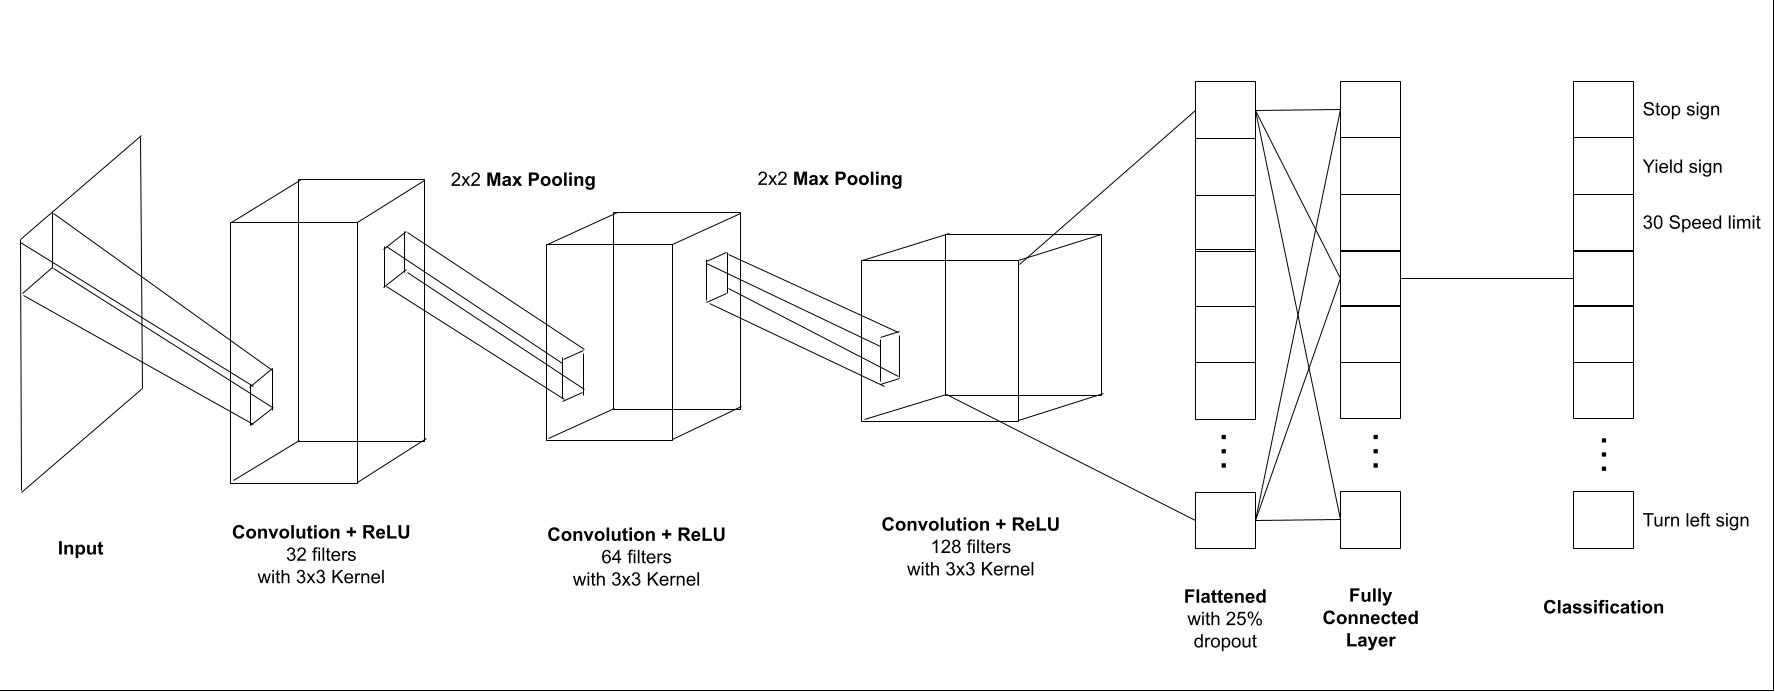
\includegraphics[width=\textwidth]{Figs/DiagramCNN.png}
\end{center}
\caption{Diagram of current CNN model}
\end{figure}

\subsubsection{Convolutional Layers}
The core of our architecture is a series of convolutional layers, each followed by ReLU (Rectified Linear Unit) activations. These layers are designed to capture various visual features, such as edges, colors, and shapes. Each convolutional layer has multiple filters that apply convolution operations on the image, progressively learning more abstract features. For instance, early layers capture low-level details like edges and textures, while deeper layers focus on high-level structures such as traffic sign shapes. We use the ReLU activation function, which introduces non-linearity and helps the network learn complex patterns without the risk of gradient vanishing.

\subsubsection{Layer Configuration:}
\begin{itemize}
    \item First Block: 32 filters, 3x3 kernel
    \item Second Block: 64 filters, 3x3 kernel
    \item Third Block: 128 filters, 3x3 kernel
\end{itemize}

\subsubsection{Pooling Layers}
Between each convolutional layer, we added a 2x2 max-pooling layer to downsample the feature maps and reduce the spatial dimensions, while retaining the most significant feature within that region. Pooling helps in reducing computation and minimizing the risk of overfitting by focusing on the most crucial features while discarding less important details.

\subsubsection{Dropout Layers}
To address potential overfitting, particularly when working with a limited dataset, dropout layers are introduced after each pooling layer. These layers randomly deactivate a proportion of neurons during training, forcing the network to reduce dependency on specific neurons. We applied a dropout rate of 25%. 

\subsubsection{Fully Connected Layers and Output Layers}
After flattening the final pooled feature map, the data is fed into fully connected (dense) layers, where high-level reasoning occurs. These layers serve to interpret the abstracted features from convolutional layers and perform classification. The model includes a dense layer with 128 units and ReLU activation, followed by a dropout of 50\% to prevent overfitting.

The output layer is a dense layer with a number of neurons equal to the number of traffic sign classes in the dataset, using a softmax activation function. Softmax provides a probability distribution across the classes, meaning the model assigns a score to each class prediction.

\subsubsection{Training Analysis}
For the training loop, we used an Adam optimizer and a Cross Entropy loss function. We chose the Adam optimizer as it has low memory usage and the cross entropy function as its ideal for multi-class classification. We trained using a batch size of 64, learning rate of 0.01, and 20 epochs. The training and validation accuracy curves (see Figure 8) indicate steady learning with no major signs of overfitting or underfitting, demonstrating that the architecture is well-suited to the problem. The current model was able to reach a training accuracy of 95.45\% and a validation accuracy of 92.35\%. The loss curves (Figure 9) show a similar trend, with validation loss converging closely with training loss over epochs.

\begin{figure}[h]
\begin{center}
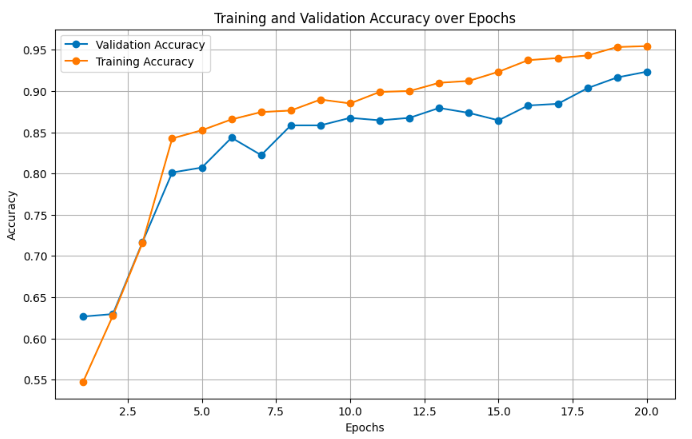
\includegraphics[width=\textwidth]{Figs/Accuracy Graph.png}
\end{center}
\caption{Training and Validation Accuracy over Epochs.}
\end{figure} 
\newpage


\begin{figure}[h]
\begin{center}
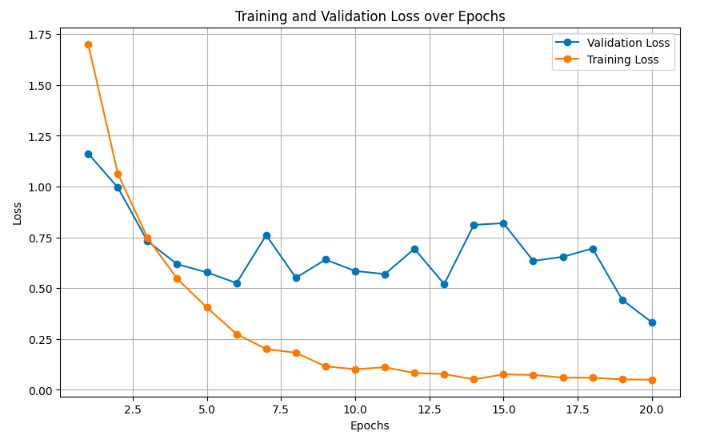
\includegraphics[width=\textwidth]{Figs/Loss Graph.png}
\end{center}
\caption{Training and Validation Loss over Epochs.}
\end{figure} 

When evaluated on specific sample classes, the model was particularly effective at recognizing common signs (ex. speed limits), which are crucial for driving safety. However, it struggled more with less common signs that have lower representation in the dataset. This means that we have a class imbalance that might lead to biased predictions toward more frequent traffic signs. This suggests the system would benefit from more data or data augmentations specifically focused on those rare classes.


\section{References}

\label{last_page}

\bibliography{APS360_ref}
\bibliographystyle{iclr2022_conference}

\end{document}
